\documentclass[swedish]{beamer}
\usetheme{Hannover}
\usecolortheme{beetle}
\usepackage{paratype}
\renewcommand*\familydefault{\sfdefault}
\beamertemplatenavigationsymbolsempty

\usepackage{tikz}
\usepackage{tikz-qtree}
\usepackage{pgf-umlsd}

\usetikzlibrary{trees,angles,arrows,calc,arrows, shapes, positioning,intersections}
\tikzset{
	class/.style={rectangle,
		draw=blue!70,
		fill=blue!20,
		rounded corners,
		minimum size=8mm,
		},
	constraint/.style={circle,
		draw=orange!70,
		fill=orange!20,
		},
	classclass/.style={rectangle,
		draw=blue!70,
		fill=blue!20,
		rounded corners,
		rectangle split,
		rectangle split parts=3,
		font=\scriptsize \ttfamily
		},	
	attribute/.style={rectangle,
		draw=yellow!70,
		fill=yellow!20,
		font=\tiny \ttfamily,
	},
	edge from parent/.style={draw},
	edge from parent path={(\tikzparentnode.south) -- (\tikzchildnode.north)},
	every node/.style={font=\footnotesize \sffamily},
	mandatory/.style={edge from 					
			parent/.style={draw,-*}},
	optional/.style={edge from 					
				parent/.style={draw,-o},
				},
	attrOf/.style={dashed, ->},
	normal/.style={edge from parent/.style={draw},
	},
	inherits/.style={->, >=open triangle 90, thick},
	assoc/.style={-diamond}
}



\title[Configuration Testing]{SMT Aided Test Case Generation For Constrained Feature Models}


\institute[LiU]{Link\"opings University, Ericsson AB}
\date{\today}


\begin{document}
\author[Paul Borek]{Paul Borek\\\vspace{1em}\begin{tabular}{r@{ }l}
Supervisors: & Ahmed Rezine (LiU) \\
	         & Johan Moe (Ericsson AB)\\
Examiner: & Kristian Sandahl (LiU)
\end{tabular}}

 \begin{frame}
  \titlepage
 \end{frame}
 
 \begin{frame}
  \frametitle{Introduction and Motivation}
  \begin{itemize}
   \item Highly configurable systems
   \item Additional testing (scenarios for other testing activities and Configuration manager)
   \item Involved constraints
   \item Testing: creating configurations which satisfy the constraints.
   \item Manually/hard-coded: fixed scenarios, but not interesting to test the configuration manager.
  \end{itemize}
 \end{frame}
 
 \begin{frame}
  \frametitle{Goal}
  \begin{itemize}
   \item Desired: automation of configuration testing.
   \item Input: Configuration description, additional information.
   \item Output: set of configurations
   \item Postconditions: coherent wrt constraints.
   \item coherent wrt. configuration description.
  \end{itemize}
 \end{frame}

 \begin{frame}
  \frametitle{Project Context}
  \begin{enumerate}
   \item Masterthesis was elaborated at Ericsson Link\"oping.
   \begin{itemize}
    \item Fixed and mobile broadband solutions.
    \item Business and operations support.
    \item 2G/3G/4G mobile network infrastructure.
   \end{itemize}
   
   \item Current project involves about 200 developers in Link\"oping as well as other subsidiaries in Stockholm and Anyang, South Korea.
   
   \item Long-term project with focus on many customers and even more users. 
  \end{enumerate}
 \end{frame}
 
 \begin{frame}
  \frametitle{Modeling Variability at Ericsson AB}
  \begin{itemize}
   \item \emph{Ericsson Common Information Model (ECIM)}
   \item Support of operations and maintenance on Managed Object.
   \item Managed Object is conceptual view of network resource (network component, host system or application).
   \item For our purpose: they describe the allowed configuration of the end-system.
   \item 
 \end{frame}
 
 \begin{frame}
  \frametitle{Feature Models}
  \begin{enumerate}
   \item Identify product functionality by referring to re-usable assets (\emph{features}) for developers \emph{and} stakeholders in the same way.
   \item Represent those features as a \emph{feature diagram}:
    \begin{itemize}
     \item Features as nodes.
     \item Different containment relations:
     \begin{itemize}
      \item \emph{Mandatory} features.
      \item \emph{Optional} features.
      \item \emph{Alternative} feature groups.
      \item \emph{Or-relation} feature groups.
     \end{itemize}
     \item Basic constraints:
     \begin{itemize}
      \item \emph{Requires:} Feature $A$ requires feature $B$ if feature $B$ has to be included whenever $A$ is included in the final diagram.
      \item \emph{Excludes:} Feature $A$ excludes feature $B$ if both features cannot appear in the same product
     \end{itemize}
    \end{itemize}
    \item \emph{Configuration:} end-product with chosen features.
    \end{enumerate}
   \end{frame}
   
   \begin{frame}
   \frametitle{Example Feature Model}
   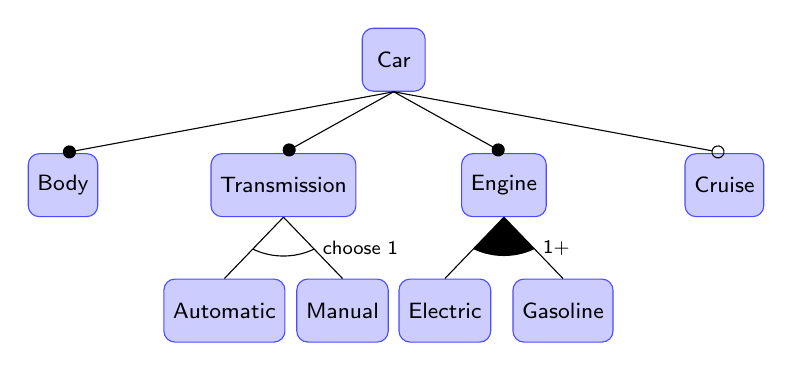
\begin{tikzpicture}[level distance=2cm,
   	level 1/.style={sibling distance=2.8cm},
   	level 2/.style={sibling distance=1.5cm, 
   		level distance=2cm},
   	]
   
   \node[class] (car) {Car} [anchor=south]
   	child[mandatory] { node [class, mandatory] (body) {Body}}
   	child[mandatory] { node [class, mandatory] (transmission) {Transmission} 
   		child[normal] { node [class] (auto) {Automatic}}
   		child[normal] { node [class] (manual) {Manual}
   		edge from parent node [right] {\scriptsize choose 1}}
   		}
   	child[mandatory] { node [class, mandatory] (engine) {Engine}
   		child[normal] { node [class] (electric) {Electric}}
   		child[normal] { node [class] (gasoline) {Gasoline}
   		edge from parent node [right] {\scriptsize 1+}}
   		}
   	child[optional] { node [class] (cruise) {Cruise}}
   	;
   	
   \begin{scope}
    \path[clip] (electric.north) -- (engine.south) -- (gasoline.north);
    \fill[black] (engine) circle (9mm);
   \end{scope}	
   
   \begin{scope}
    \path[clip] (auto.north) -- (transmission.south) -- (manual.north);
    \draw[black] (transmission) circle (9mm);
   \end{scope}	
   \end{tikzpicture}
   \begin{enumerate}
   \item \emph{Configuration:} Car(Body, Transmission(Automatic), Engine(Gasoline))
      \item \emph{Staged Configuration:} process of deriving a configuration.
   \end{enumerate}
   
  \note{say: features=nodes, edges=part-of, different relations}
 \end{frame}
 
 
 \begin{frame}
  \frametitle{Extensions and Constraints of feature models}
  \begin{enumerate}
   \item \emph{Attributes} add information to features. Are defined by a name, a type and a value (in a configuration)
   \item \emph{Cardinalities} are alternative representations of relations by refining them into $[n..m]$ with
   \begin{itemize}
    \item $n$ lower bound
    \item $m$ upper bound
   \end{itemize}
    
   \item \emph{Analyses} of feature models determine various metrics of feature models, i.e, number of products, variability, commonality, normalizations etc.
  \end{enumerate}
 \end{frame}
 
 \begin{frame}
 \frametitle{Back to Ericsson}
 \begin{enumerate}
  \item \emph{Ericsson Common Information Model (ECIM)} describes a conceptual view of a resource, such as a network component, host system or application. Composed of a set of \emph{management information model (MIM)} files.
  
  \item \emph{Feature} has been replaced with \texttt{class}, which is uniquely identified by its \texttt{mim}-name (name-space) and the class-name and consists of 
   \begin{itemize}
    \item \emph{key-attribute} of type \texttt{string} is the unique identifier of an instance.
    \item a set of \texttt{attributes}, which have a name and a data-type.
   \end{itemize}
  
  \item \emph{parent-child relations} with cardinalities.
  
  \item \emph{bi-directional associations} with a \emph{server} and a \emph{client}. Server contains reference to client, i.e., path from root node to client. 
 \end{enumerate}
 \end{frame}
 
 \begin{frame}
  \frametitle{Constraints in ECIM}
  \begin{enumerate}
   \item Constraints (or dependencies) are defined on a class.
   \item Currently \emph{Schematron} is used.
   \item Schematron is a validation language for XML documents. 
   \item Uses a reduced set of XPath expressions to encode constraints.\note{reduced in the number of available functions}
  \end{enumerate}
 \end{frame}
 
 %TODO methodology: as inside the 
 \begin{frame}
 \frametitle{Methodology}
 \begin{enumerate}
  \item Goal and Scope.
  \item Subdivision of the problem.
  \item Investigation of the different parts.
  \item Implementation
 \end{enumerate} 
 \end{frame}
 
 \begin{frame}
  \frametitle{Goal and Scope.}
  \begin{itemize}
   \item Create test-cases in order to apply traditional testing techniques on different configurations.
   
   \item Constraint satisfaction of the test-cases has highest priority.
   
   \item Rather interested in a small set of coherent test-cases instead of a big suite with a high interaction coverage.
   
   \item Outcome: besides theoretical considerations a tool to produce test-cases.
   
   \item Development of external, user-defined annotations to guide the test-case generation.
  \end{itemize}
 \end{frame}
 
 \begin{frame}
  \frametitle{Subdivision of the Problem}
  \begin{itemize}
   \item Test-case: instances of classes with attribute-values which respect the parent-child relations and constraints.
   \item Test-suite: set of test-cases which should respect certain objectives.
   \item 3 facets of the overall problem:
    \begin{enumerate}
     \item Structural properties: tree-construction and cardinalities (number of instances). 
     \item Constraints.
     \item Unconstrained attributes.
    \end{enumerate}
  \end{itemize}
 \end{frame}
 
 \begin{frame}
  \frametitle{Structural Properties}
  \begin{itemize}
   \item Creation of the tree by selecting instances.
   \item Approach: Czarnecki et. al. define \emph{staged configuration} as the subsequent generation of a end-product in each stage by choosing values from a cardinality-range.
   
   \item No algorithm specified.
   \item To achieve a desired \emph{structural coverage}, choose \emph{skip-factor}, which indicates those cardinalities which are omitted:
   \begin{block}{Skip-factor-based staged configuration}
   Cardinality of class $\mathcal{C}$: $I(\mathcal{C})=[n..m]$, chosen number $c$\\
   Start with one test-case where $c := n$.
   Then increment $c$ by $x$ with
   \[
   x = \lceil (\max{I(\mathcal{C})}-\min{I(\mathcal{C})}) \rceil * \sigma
   \]
   until $c = m$, where $\sigma$ is the user defined \emph{skip-factor}.
   \end{block}
  \end{itemize}
 \end{frame}
 
 \begin{frame}
  \frametitle{CSP and SAT}
  \begin{enumerate}
   \item Constraint Satisfaction Problems:
    \begin{enumerate}
     \item set of variables.
     \item set of constraints.
     \item each variable has a domain of possible values.
     \item each constraint involves some subset of variables and specifies the allowable combinations of that subset.
     \item A solution assigns every variable in the CSP a value while satisfying the constraints.
    \end{enumerate}
   \item Problem is NP-hard.
   \item Most famous (boolean) CSP: satisfiability of propositional logic (SAT).
    \begin{itemize}
     \item Benefit: fastest CSP solver.
     \item Drawback: input language (encoding), nature of real world problems (sets, arrays, declarative data-types) do not provide good encodings.
    \end{itemize}
   \item split boolean reasoning procedures from other theories, which do not provide good encodings: sat modulo theory.
  \end{enumerate}
 \end{frame}
 
 \begin{frame}
  \frametitle{SAT modulo theory}
  \begin{enumerate}
   \item Uses \emph{first order logic} instead of propositional logic: adds more power in terms of Quantifiers, Functions and predicates.
   \item Uses Background theories: constrains the interpretation of some functions and predicates.
   \item A formula $\phi$ is satisfiable modulo a theory $T$, if $M \models_{T} \phi$. $M$ is called a model which satisfies $T \cup \{\phi\}$.
   \item A procedure $\mathfrak{S}$ is called a decision procedure for $T$, if $\mathfrak{S}$ can check whether any quantifier-free formula is satisfiable or not. In this case $T$ is called decidable.
   
   \item Big variety of decision procedures for: arithmetic, free functions, bit-vectors, arrays.
  \end{enumerate}
 \end{frame}
 
 \begin{frame}
  \frametitle{From theory to the MIM model.}
  \begin{enumerate}
   \item in MIM models, constraints play a major role. 
   
   \item 
  \end{enumerate}
 \end{frame}
\end{document}